\section{Versuchsdurchführung}
\subsection{Durchlassfilter als Frequenzfilter}
Zur Überprüfung der Funktionsweise eines Frequenzfilters wurde zunächst die Schaltung aus
Abb. \ref{plan:durchlass} auf Seite \pageref{plan:durchlass} wie in Abb. \ref{img:durchlass} realisiert. Nach anfänglichen Problemen mit der richtigen Dimensionierung der verwendeten Spule haben wir hier schließlich eine Spule "Leybold 56214" mit 500 Windungen und einer Induktivität von 9 mH verwendet, wobei das Augenmerk auf einer möglichst geringen Windungszahl liegt, um den in der Spule angesiedelten Widerstand möglichst gering zu halten. Dieser liegt für die Spule bei angegebenen 2,5 $ \Omega $, was durch Messung bestätigt wurde. Auf
der anderen Seite musste auch eine hinreichend große Induktivität garantiert werden, damit die Resonanzfrequenz, in deren Umgebungen die Messungen stattfanden, in einem gut erfassbaren Bereich lagen. Weiter wurde ein Plastikfolienkondensator der Firma "WIMA" der Kapazität 0,22 $  \mu F $ sowie in einem zweiten Teilversuch ein Kondensator gleicher Bauart, allerdings mit 4,7 $  \mu F $ Kapazität verwendet. Da beide Teilversuche übereinstimmende Ergebnisse lieferten, wird in der Auswertung nur der erste Teilversuch dargestellt. Weiter wurde der Widerstand als variabel gewählt, wobei hier ein
Widerstandskasten, mit dem Widerstände im Bereich von 1 $ \Omega $ bis mehrere $M \Omega $ zugeschaltet werden können, verwendet wurde. \\
Zur Erzeugung der Eingangsspannung wurde zunächst ein Frequenzgenerator der Marke Hameg (Programmable 15 MHz Function Generator, HM8131/2) verwendet, zur Vereinfachung und Automatisierung der Messung wurde dieser allerdings durch das Power-Cassy ersetzt.
Die Messung der über dem Widerstand abfallenden Ausgangsspannung wurde bei einem ersten Aufbau mit einem Oszilloskop (Tektronix TDS 2024 100mHz, PPL28/2/001) durchgeführt. Hierbei stellte sich allerdings heraus, dass die Messungen etwas an Genauigkeit zu wünschen übrig ließen. Bei der tatschlichen Durchführung des Experiments haben wir stattdessen das Sensor-Cassy zugeschaltet; Vorteil hierbei ist klar die direkte Übertragung der Daten in die Cassy-Software.

\begin{figure}[h]
\centering
    \subcaptionbox{Durchlassfilter\label{img:durchlass}}[.4\linewidth]
            {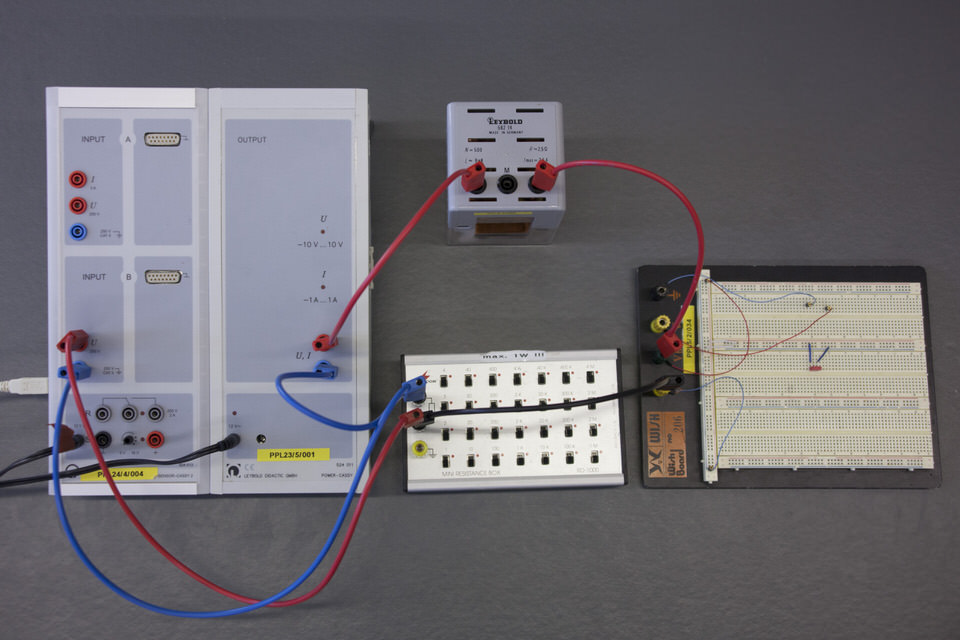
\includegraphics[width=.4\textwidth]{images/durchlassfilter.jpg}}
    \subcaptionbox{Sperrfilter\label{img:sperr}}[.4\linewidth]
            {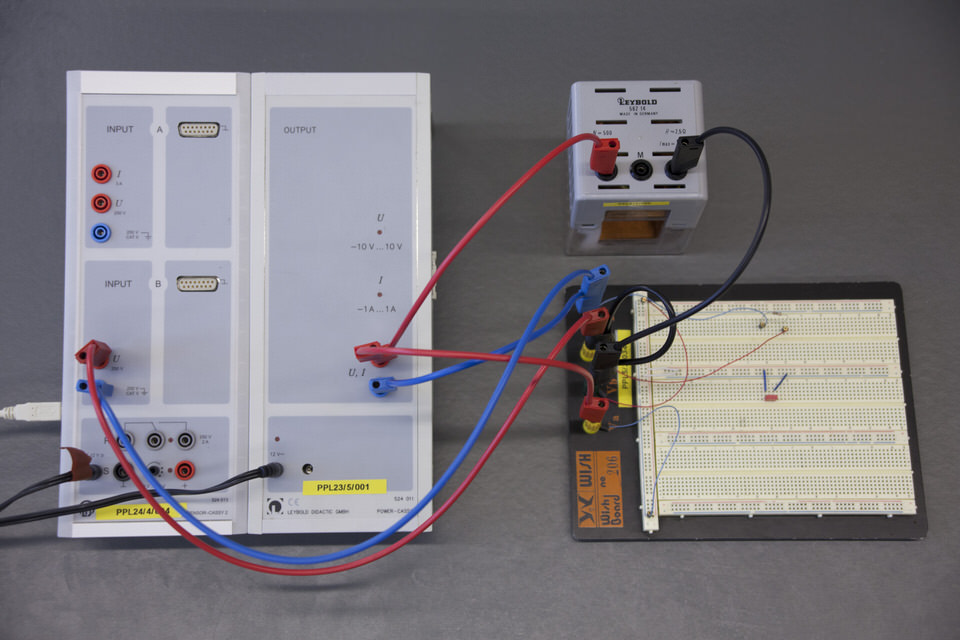
\includegraphics[width=.4\textwidth]{images/sperrfilter.jpg}}
\caption{Fotos der Versuchsaufbauten}
\end{figure}

\subsection{Sperrfilter als Frequenzfilter}
Für die Abwandlung des Durchlassfilters zu einem Frequenzfilter müssen lediglich Kapazität und Induktivität parallel anstatt in Reihe geschaltet werden, wie in Abb. \ref{plan:sperr} dargestellt. Für diesen Versuch wurde der zweite Kondensator mit einer Kapazität von 4,7 $  \mu F $ sowie daneben eine Spule höherer Induktivität (36 mH bei 1000 Windungen; ebenfalls von "Leybold") verwendet. Grund hierfür war eine erwartetet Senkung der Resonanzfrequenz und eine damit verbundene bessere Messung. Tatsächlich wurde aber kein qualitativer Unterschied zum Durchlassfilter und ersterer Spule 
bei der Genauigkeit der Messung erzielt. Um für dieses Experiment den teilweise recht schwach ausgebildeten Peak deutlicher sichtbar zu machen, also eine geringere Breite zu erreichen, wurde weiter die Widerstandsbox durch einen einfachen Steckwiderstand, wie etwa in Abb. \ref{img:sperr} zu sehen
ersetzt. Grund dafür ist, dass die Widerstandsbox insbesondere bei den kleinsten Widerständen einen zu großen tatsächlichen Widerstand liefert.



